\subsection{CouchDB} \label{couchdb}
CouchDB is an open-source database software that provides capability to store document-oriented structures in multi-node environment. The entire couchdb environment setup is managed by \texttt{sds-deps-install-couchdb} and \texttt{sds-deploy-couch-cluster} roles.

\subsubsection{Installation}
CouchDB installation is one the most critical component of the entire project, since it will be used by the harvester and application for showing our story. For installation, we have used source-based installation approach. In this approach, we download CouchDB source-code from Apache servers and build it using \texttt{make} command. This entire flow is implemented and executed using \texttt{Ansible}.

\begin{figure}[H]
    \centering
    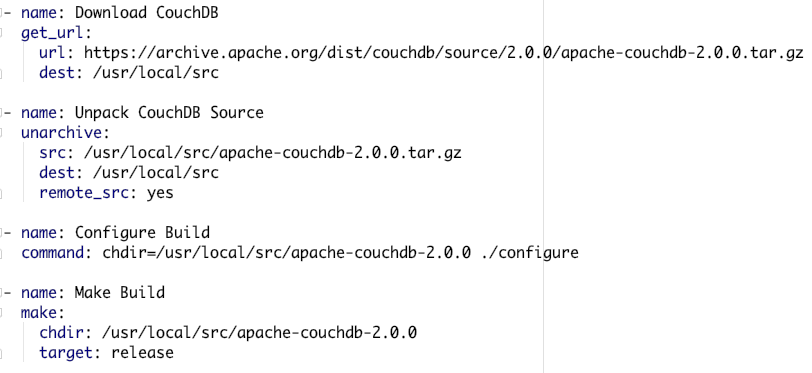
\includegraphics[width=12cm,keepaspectratio=true]{images/deployment/couchdb_installation.png}
    \caption{Downloading and installing CouchDB from source}
    \label{fig:couchinstallation1}
\end{figure}

\subsubsection{Configuration}
After CouchDB is build from the source successfully, following steps are required to configure it as expected:

1. Add CouchDB account in the system

2. Change ownership of folder where CouchDB is installed - \texttt{770 mode} 

3. Change node name in \texttt{/couchdb/etc/vm.args} from localhost to server's IPv4 address.

4. Add kernel arguments in \texttt{/couchdb/etc/vm.args} for enabling couch cluster setup.

5. Set unique cookie in \texttt{/couchdb/etc/vm.args} for establishing membership with other nodes. This unique cookie is same in all nodes of the CouchDB by which cluster can be established.

6. Bind node address \texttt{chttpd} to \texttt{0.0.0.0:5990} so that it can be accessible from outside.

7. Install CouchDB service in \texttt{/etc/systemd} and set it to start during system startup.

\begin{figure}[H]
    \centering
    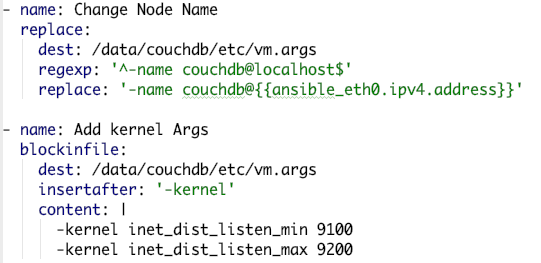
\includegraphics[width=6cm,keepaspectratio=true]{images/deployment/couchdb_config.png}
    \caption{Configuring node and kernel of CouchDB using Ansible}
    \label{fig:couchinstallation2}
\end{figure}

\subsubsection{Cluster Setup}
After CouchDB is properly configured, it should be up and running on all the provided virtual machines. Now, we need to connect all nodes into a cluster so as to use sharding and replication features of CouchDB. Using \texttt{sds-couch-nodes-cluster} Ansible package, we can create cluster of CouchDB depending upon the master node provided in \texttt{hosts\_couch} file and child nodes provided in \texttt{sds-couch-dynamic-vars.yaml}. As stated before, these files are generated by the \texttt{sds-infra} package and placed into their respective location by the main executing script. We can create CouchDB nodes cluster using following steps, which are executed by the master node:

1. Register all child nodes that are going to be a part of the cluster by using \texttt{cluster\_setup} API with action \texttt{enable\_cluster}.

2. Add all child nodes into the cluster by using the same API with action \texttt{add\_node}.

3. After all child nodes are added into the cluster, master node can complete cluster setup by using the same API with action \texttt{finish\_cluster}.

\begin{figure}[H]
    \centering
    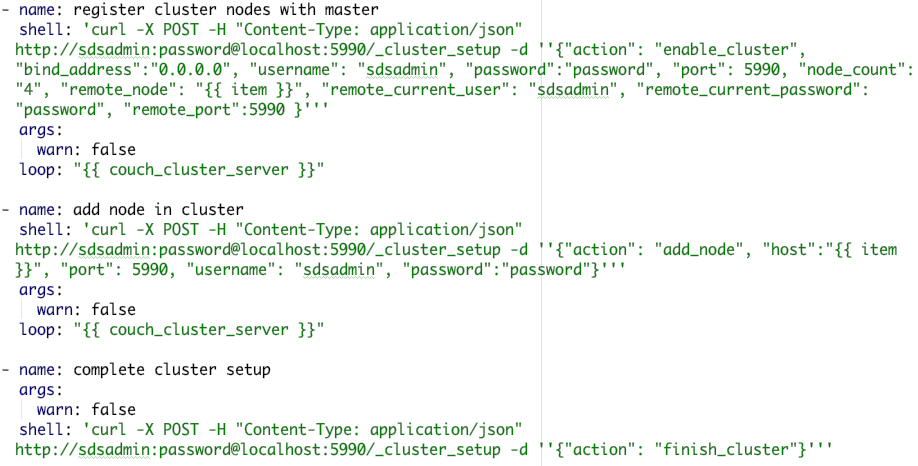
\includegraphics[width=12cm,keepaspectratio=true]{images/deployment/couch_cluster_setup.png}
    \caption{CouchDB cluster setup using Ansible}
    \label{fig:couchinstallation3}
\end{figure}

\begin{figure}[H]
    \centering
    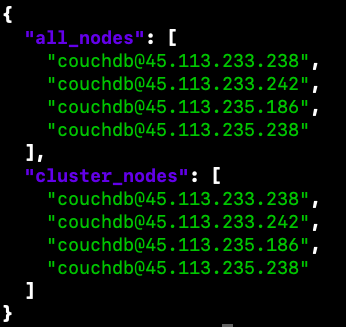
\includegraphics[width=5cm,keepaspectratio=true]{images/deployment/couchdb_cluster.png}
    \caption{CouchDB current cluster membership (4-node-4-VM)}
    \label{fig:couchinstallation4}
\end{figure}

\subsubsection{Database and View Initialization}
After completion of CouchDB cluster setup, all 4-nodes of CouchDB are communicating with each other as required. Now, we need to initialize our couch databases with their respective design documents containing view so that our UI is able to fetch data from the couch instance.

1. We create our all 3 databases with 8 shards and 3 replicas using Ansible: \texttt{sds\_db, sds\_db\_vis, sds\_processed\_users.}

\begin{figure}[H]
    \centering
    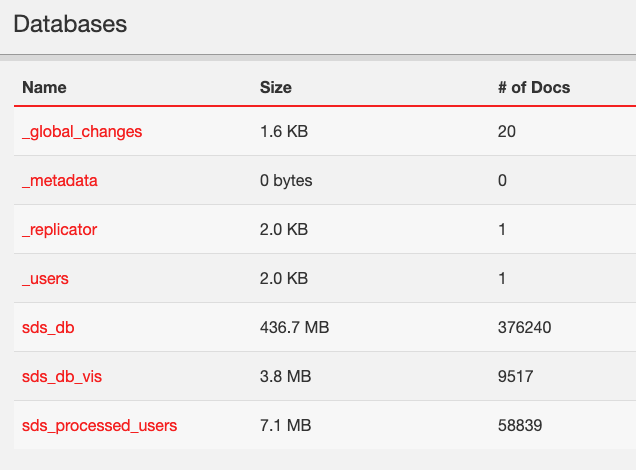
\includegraphics[width=8cm,keepaspectratio=true]{images/deployment/couchdb_databases.png}
    \caption{Databases stored in 4-node CouchDB cluster}
    \label{fig:couchdatabases}
\end{figure}

2. CouchDB views are stored in \texttt{json} file with their respective design document identifier. They are copied to the VM server which can later be deployed in their respective databases.

\begin{figure}[H]
    \centering
    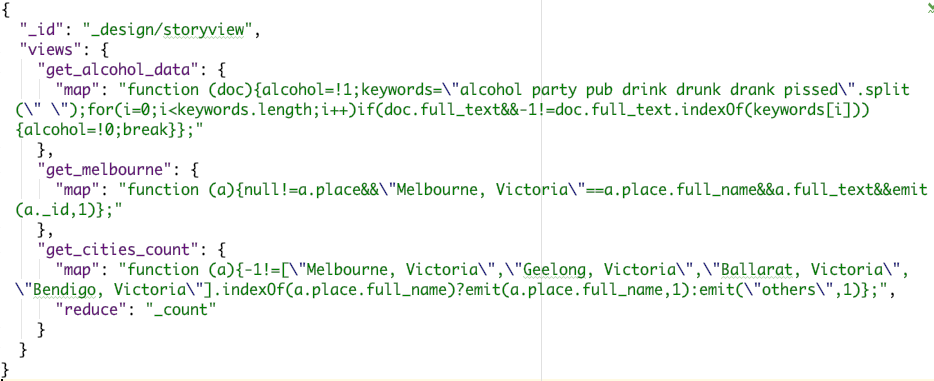
\includegraphics[width=11cm,keepaspectratio=true]{images/deployment/couchdb_view_json.png}
    \caption{Storyview design document for \texttt{sds\_db}}
    \label{fig:couchview1}
\end{figure}

3. After views are successfully transferred, respective views are implemented in their database using cURL commands.

\begin{figure}[H]
    \centering
    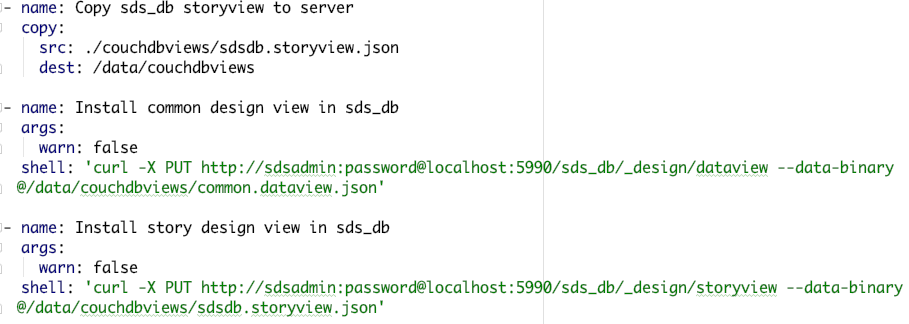
\includegraphics[width=11cm,keepaspectratio=true]{images/deployment/couchdb_view_deployment.png}
    \caption{View deployment snippet (cURL and Ansible)}
    \label{fig:couchview2}
\end{figure}
